\documentclass[11pt]{article}

% ---------------------------------------------------------------
%  The Harness Effect — token economics of agent orchestration
%  Publication draft for arXiv (cs.AI / cs.SE / econ.GN cross-list)
%  All headline numbers are centralized in the macros below so the
%  final evaluation freeze can be dropped in with one edit pass.
% ---------------------------------------------------------------

\usepackage[margin=1in]{geometry}
\usepackage{mathptmx}
\usepackage[scaled=0.92]{helvet}
\usepackage{amsmath,amssymb}
\usepackage{booktabs}
\usepackage{makecell}
\usepackage{graphicx}
\usepackage{xcolor}
\usepackage{caption}
\usepackage{microtype}
\usepackage{enumitem}
\usepackage[colorlinks=true,linkcolor=blue!55!black,citecolor=blue!55!black,urlcolor=blue!55!black]{hyperref}

\captionsetup{font=small,labelfont=bf}
\hypersetup{pdftitle={The Harness Effect: How Orchestration Design Sets the Token Economics of Enterprise Agentic AI}, pdfauthor={Writer, Inc.}}

% ----------------------- headline numbers ----------------------
\newcommand{\NP}{22}                    % prompts
\newcommand{\NM}{six}                   % models
\newcommand{\CostA}{\$0.21}\newcommand{\CostB}{\$0.12}\newcommand{\CostD}{41\%}
\newcommand{\LatA}{48\,s}\newcommand{\LatB}{27\,s}\newcommand{\LatD}{44\%}
\newcommand{\SpeedX}{1.8$\times$}
\newcommand{\TokA}{14.2k}\newcommand{\TokB}{8.8k}\newcommand{\TokD}{38\%}
\newcommand{\QA}{0.78}\newcommand{\QB}{0.81}
\newcommand{\QPDgain}{82\%}
\newcommand{\CPMA}{54.9}\newcommand{\CPMB}{92.0}\newcommand{\CPMgain}{68\%}
\newcommand{\CostRange}{33\% to 61\%}
\newcommand{\FreezeDate}{2026-06-07}
% ----------------------------------------------------------------

\title{\LARGE\bf The Harness Effect: How Orchestration Design Sets\\[2pt] the Token Economics of Enterprise Agentic AI}

\author{\parbox{0.94\textwidth}{\centering
Muayad~Sayed~Ali, Aliaksandra~Novik, Anji~Boddupally, Artem~Yavorskyi, Chris~Nickerson, Daniel~Rica, Emily~DuGranrut, Felix~Leung, Garrett~Prince, Grace~Barnett, Heath~Robinson, Hosain~Al~Ahmad, Jesse~Resnick, Juan~Carlos~Farah, Jyothi~Swaroop~Meruga, Leonid~Kuznetsov, Brock~Perry, Luke~Gorham, Marie~Schmoll, Michael~Paciullo, Saumya~Das, Sharath~Sheripally, Tommy~Griscom, Mykyta~Osadchyi, Neha~Mantri, Nick~Westrum, Olivia~Benowitz, Parikshith~Kulkarni, Radik~Chernyshov, Rakshith~Vasudev, Rohith~Nadimpally, Vikas~Gangadevi, and Waseem~AlShikh\\[9pt]
Writer, Inc.\\[3pt]
{\small\texttt{\{muayad, aliaksandra, anji, artem, chris, daniel, emily, felix, garrett, grace, heath, hosain, jesse, juan, jyothi, leonid, brock, luke, marie, michael, saumya, sharath, tommy, mykyta, neha, nick, olivia, parikshith, radik, rakshith, rohith, vikas, waseem\}@writer.com}}
}}

\date{July 2026}

\begin{document}
\maketitle

\begin{abstract}
The dominant pattern in agentic AI development is what we call \emph{token maxing}: buying capability with tokens---longer reasoning traces, more agent turns, wider tool payloads, larger replayed contexts---so that tokens per task grow faster than task value. Falling per-token prices mask the pattern without fixing it; total spend rises anyway. We argue that the decisive lever against token maxing is the \emph{harness}: the orchestration layer that assembles context, exposes tools, sequences turns, delegates work, and carries the observability and governance surface an enterprise deployment runs on. To isolate this layer we run a controlled swap: the same \NP{} locked evaluation tasks on the same \NM{} foundation models (Claude Sonnet~4.6, Gemini~3.1, Gemini Flash~3.5, Qwen~3.6, GLM~5.1, and Palmyra~X6), changing only the orchestration layer: a conventional production agent loop (the frozen baseline) versus the Writer Agent Harness. Holding models constant, placing the harness at the core of execution cuts blended cost per task by \CostD{} (\CostA{}~$\rightarrow$~\CostB{}), median wall-clock by \LatD{} (\LatA{}~$\rightarrow$~\LatB{}), and tokens per task by \TokD{} (\TokA{}~$\rightarrow$~\TokB{}), while headline task-completion quality holds at parity (\QA{}~$\rightarrow$~\QB{}, directional at this sample size). The efficiency gains are \emph{model-invariant}---every model gets cheaper, by \CostRange{}---while quality gains are \emph{capability-dependent}: the improvement a model extracts from the harness correlates almost perfectly with its baseline strength ($r=0.99$, $n=6$), a phenomenon we term \emph{harness leverage}. Quality per dollar rises \QPDgain{} and task-completions per million tokens rise from \CPMA{} to \CPMB{}. On this workload, the orchestration layer moved cost per task more than switching between the cheapest and most expensive model did. We formalize token economics at the orchestration layer, including an effective-input-price model under prompt caching; define token maxing; detail the six mechanism families behind the effect, from cache-shape discipline to failure-spend governance; compare six widely used agent systems on the same axes; and argue that the harness is the one component whose efficiency multiplies across every model an organization runs---present and future.
\end{abstract}

\section{Introduction}
\label{sec:intro}

An agentic task is not one model call. A single request---``reconcile these two contracts and draft the redline memo''---unfolds into a dozen or more turns: system prompt, tool schemas, retrieval payloads, intermediate reasoning, tool outputs, and, in naive implementations, the full replay of everything above on every subsequent turn. The token bill for the task is the sum over that loop, and the loop is governed not by the model but by the software around it. We call that software the \emph{harness}: the orchestration layer that decides what enters the context window, which tools are visible, when to retrieve, when to retry, when to delegate, and when to stop.

The industry's default response to rising agent capability requirements has been to spend more tokens. Reasoning models emit thousands of deliberation tokens per answer; agent frameworks replay conversation history quadratically in the number of turns; tool ecosystems inject every schema into every call. Per-token prices have fallen steadily \cite{epoch2025}, and the falling unit price has financed the habit: teams treat tokens as nearly free at the margin and scale consumption to match. This is a textbook Jevons dynamic---efficiency gains in the resource lower its price and raise total consumption \cite{jevons1865}---and it produces a development trajectory we name \textbf{token maxing}: quality is purchased with monotonically growing token intensity, at declining marginal quality per token (Definition~1, Section~\ref{sec:framing}). Token maxing is invisible in benchmark tables, which report quality, and painfully visible in cloud invoices, which report tokens.

Most published efficiency work attacks this problem \emph{inside} a single model call---prompt compression \cite{llmlingua}, budget-constrained reasoning \cite{tale}, terse decoding \cite{cod}, speculative decoding \cite{spec}, serving-side memory management \cite{vllm}---or \emph{between} models, by routing and cascading \cite{frugalgpt,routellm}. Both families accept the orchestration layer as given. Yet the harness controls every term of the token bill except the model's own verbosity: the system prompt is replayed or cached by the harness; history is replayed or compacted by the harness; tool schemas are broadcast or scoped by the harness; retrieval payloads are sized by the harness; retries are triggered by the harness. If the harness is the layer that composes model calls into work, it is also the layer that sets the price of work.

This paper measures that claim directly with a natural experiment the layered architecture makes possible: \textbf{hold the tasks and the models constant, and swap only the orchestration layer}. We evaluate \NP{} locked, capability-audited enterprise tasks on \NM{} foundation models spanning five vendors and three weight classes, under two orchestration layers: a conventional production agent loop, frozen on \FreezeDate{} as the baseline, and the Writer Agent Harness, a model-agnostic orchestration layer with sub-agent delegation. Every task, prompt, model identifier, judge, and price table is identical across the two arms; the only variable is the orchestration code.

\medskip
\noindent The headline results (Section~\ref{sec:results}):

\begin{enumerate}[leftmargin=1.6em,itemsep=2pt]
\item \textbf{Efficiency moves a lot, and it moves everywhere.} Blended across models, cost per task falls \CostD{} (\CostA{}~$\rightarrow$~\CostB{}), median wall-clock falls \LatD{} (\LatA{}~$\rightarrow$~\LatB{}; \SpeedX{} faster), and tokens per task fall \TokD{} (\TokA{}~$\rightarrow$~\TokB{}). The per-model cost reduction ranges from $-$33\% (Gemini~3.1) to $-$61\% (Flash~3.5): \emph{every} model gets substantially cheaper. On this workload the harness is a bigger cost lever than model choice: moving from the most to the least expensive model under the baseline saves 36\%, while keeping any model and adopting the harness saves \CostRange{}.
\item \textbf{Quality holds---and where it moves, it moves with the model.} Headline task-completion is \QA{}~$\rightarrow$~\QB{} (a wash at $n=\NP$). Across the 48 capability$\times$model cells, 30 improve, 11 are flat, and 7 regress; all 7 regressions occur on the three smaller models, concentrated in orchestration-heavy capabilities (tool use via MCP, multi-step Playbooks). The mean quality gain a model extracts from the harness tracks its baseline strength almost perfectly ($r=0.99$): stronger models convert harness structure into quality; weaker models can be overwhelmed by it. We call this \emph{harness leverage} (Section~\ref{sec:leverage}).
\item \textbf{Efficiency and capability are not a trade this time.} Quality per dollar rises \QPDgain{}; task-completions per million tokens rise from \CPMA{} to \CPMB{} ($+$\CPMgain{}). The harness also adds one net-new capability---delegated sub-agents---which crosses a usable reliability threshold only on the two strongest models (0.85--0.86), a concrete instance of the capability floor that harness features carry.
\end{enumerate}

\medskip
\noindent\textbf{Contributions.}
(1)~A formal framing of token economics at the orchestration layer, including a decomposition of per-task token spend into harness-controlled terms, an effective-input-price model under prompt caching, and a definition of token maxing as a measurable development trajectory (Section~\ref{sec:framing}).
(2)~A controlled harness-swap methodology that isolates orchestration effects from model effects, with a locked task set, frozen baseline, and trace-level accounting (Section~\ref{sec:setup}).
(3)~Empirical findings across \NM{} models: model-invariant efficiency gains, capability-dependent quality gains (harness leverage), and a capability floor for advanced orchestration features (Section~\ref{sec:results}).
(4)~A mechanism inventory of the harness---cache-shape discipline, structured compaction, context offload, zero-token waiting, failure-spend governance, and a model-agnostic floor---mapped onto the cost decomposition, together with an architectural comparison of six widely used agent systems on the same axes (Sections~\ref{sec:mechanisms}--\ref{sec:landscape}).
(4)~An economic analysis of why harness efficiency compounds---it multiplies against every model, every vendor migration, and every unit of volume---and what that implies for the own-versus-rent decision on orchestration infrastructure (Section~\ref{sec:discussion}).

\section{Related Work}
\label{sec:related}

\paragraph{Model-side and serving-side efficiency.} A large literature reduces the cost of a \emph{given} sequence of tokens: speculative decoding accelerates autoregressive generation without changing outputs \cite{spec}; PagedAttention and related memory managers raise serving throughput \cite{vllm}. These techniques lower the price of a token. They do not reduce how many tokens an agent decides to consume, which is the quantity this paper targets.

\paragraph{Prompt-side token reduction.} LLMLingua and successors compress prompts while preserving task performance \cite{llmlingua}; token-budget-aware reasoning constrains deliberation length \cite{tale}; Chain-of-Draft shows that terse intermediate reasoning can match verbose chain-of-thought \cite{cod,cot}. These methods operate within one call. An agent harness invokes such calls dozens of times per task and adds cross-call structure---history replay, tool schemas, retrieval---that no single-call method sees. Our results indicate the cross-call structure is where the larger savings sit: a \TokD{} reduction in tokens per task achieved with no change to models or prompts.

\paragraph{Routing and cascades.} FrugalGPT and RouteLLM cut cost by sending easy queries to cheap models \cite{frugalgpt,routellm}. Routing chooses \emph{which} model pays the bill; the harness determines \emph{how large the bill is} for whichever model is chosen. The two are complementary, and Section~\ref{sec:codesign} argues our capability-floor finding sharpens routing: requests should be routed not only by difficulty but by the orchestration features they will exercise.

\paragraph{Agent architectures.} ReAct interleaved reasoning and tool calls \cite{react}; Reflexion added verbal self-correction \cite{reflexion}; Toolformer trained tool invocation into the model \cite{toolformer}; SWE-agent showed that the \emph{agent--computer interface} materially changes task success \cite{sweagent}; MemGPT introduced OS-style context paging \cite{memgpt}; the Model Context Protocol standardized tool connectivity \cite{mcp}. This line established that scaffolding shapes capability. Long-context studies explain one mechanism: models attend unevenly across long inputs, so bloated contexts can \emph{reduce} accuracy while raising cost \cite{lost}. We extend the scaffolding-shapes-capability result with its economic dual---scaffolding sets cost---and quantify both sides under a controlled swap.

\paragraph{Evaluation and test-time compute.} LLM-as-judge protocols \cite{judge} and locked benchmark suites \cite{swebench} underpin our measurement design. Work on optimal test-time compute allocation \cite{snell} shows quality can be bought with inference tokens; our framing treats that purchase as an economic decision with a declining marginal rate, and the harness as the buyer of record. Reflective prompt-evolution systems such as GEPA \cite{gepa} optimize the instructions a harness issues; they are natural complements that operate \emph{through} the layer we measure.

\paragraph{Economics of inference.} Scaling laws priced training compute \cite{kaplan,chinchilla}; Epoch~AI documents multi-order-of-magnitude declines in inference prices \cite{epoch2025}. Jevons observed in 1865 that efficiency in coal use raised total coal consumption \cite{jevons1865}; Section~\ref{sec:framing} argues agentic AI is mid-Jevons, and that the harness is the layer at which consumption discipline can actually be implemented.

\paragraph{The harness as first-class object.} Closest to our framing, a recent line of work elevates the harness itself to an object of study: Gu argues agentic progress is now \emph{system} scaling---context governance, memory, skill routing---as much as model scaling \cite{harnessscaling}, and Harness-Bench measures, across 5{,}194 trajectories, that completion, efficiency, and failure behavior vary substantially across model--harness configurations \cite{harnessbench}. Practitioner evidence points the same way: production context-engineering guidance treats KV-cache hit rate as the first metric of an agent \cite{manus}; provider documentation prices cached input at roughly a tenth of list \cite{promptcache}; controlled measurements show model quality degrading as input grows \cite{contextrot}; and Anthropic reports agents at ${\sim}4\times$ and multi-agent systems at ${\sim}15\times$ chat-level token consumption \cite{anthmulti}. We add the missing economic layer: a formal token-economics framing at the harness (Section~\ref{sec:framing}), the mechanism inventory that implements it (Section~\ref{sec:mechanisms}), and a controlled swap that prices it (Section~\ref{sec:results}).

\section{Token Economics at the Orchestration Layer}
\label{sec:framing}

\subsection{The bill for one agentic task}

Let a task execute as a $k$-turn agent loop. Turn $i$ submits input tokens $T^{\mathrm{in}}_i$ and receives output tokens $T^{\mathrm{out}}_i$. With input price $p_{\mathrm{in}}$ and output price $p_{\mathrm{out}}$ (per token), the task costs
\begin{equation}
C \;=\; \sum_{i=1}^{k}\Big( p_{\mathrm{in}}\,T^{\mathrm{in}}_i + p_{\mathrm{out}}\,T^{\mathrm{out}}_i \Big).
\label{eq:cost}
\end{equation}

The input side decomposes into terms the harness constructs:
\begin{equation}
T^{\mathrm{in}}_i \;=\; \underbrace{S_i}_{\text{system}} + \underbrace{H_i}_{\text{history}} + \underbrace{G_i}_{\text{tool schemas}} + \underbrace{R_i}_{\text{retrieval}} + \underbrace{U_i}_{\text{user turn}},
\label{eq:decomp}
\end{equation}
and the loop multiplies everything by retries and dead-end branches, which the harness also governs. A naive harness replays the full transcript: $H_i = \sum_{j<i}(U_j + T^{\mathrm{out}}_j + O_j)$ where $O_j$ is tool output at turn $j$. Total input tokens then grow quadratically in turn count,
\begin{equation}
\sum_{i=1}^{k} T^{\mathrm{in}}_i \;\approx\; kS \;+\; \frac{k(k-1)}{2}\,\bar m \;+\; k\bar G \;+\; \textstyle\sum_i R_i,
\label{eq:quadratic}
\end{equation}
with $\bar m$ the mean per-turn payload. A harness that compacts history, caches the invariant prefix (tool schemas included), offloads bulky tool outputs, and truncates retrieval to the evidential minimum converts the quadratic term to (approximately) linear (Figure~\ref{fig:replay}). Nothing about the model changes; the bill does.

\begin{figure}[t]
\centering
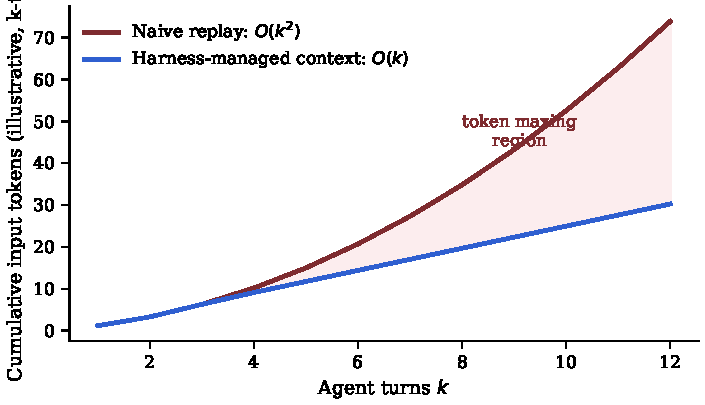
\includegraphics[width=0.62\linewidth]{figures/fig5_replay.pdf}
\caption{\textbf{Where token maxing comes from.} Illustrative cumulative input tokens for a $k$-turn agent loop. Full-history replay grows as $O(k^2)$ (Eq.~\ref{eq:quadratic}); harness-managed context---prefix caching, history compaction, offloaded tool outputs---grows as $O(k)$. The shaded gap is spend that buys no quality. Schematic; measured aggregates appear in Section~\ref{sec:results}.}
\label{fig:replay}
\end{figure}

Two further facts sharpen Eq.~\eqref{eq:cost}. First, agent workloads are \emph{input-dominated}: because the transcript is re-submitted on every turn, production agents report input-to-output token ratios near 100:1 \cite{manus}, so the $p_{\mathrm{in}}$ term is nearly the whole bill. Second, the price of an input token is not one number. Providers serve tokens that repeat a previously seen prompt prefix from cache at a deep discount---roughly $0.1\times$ the base input rate \cite{promptcache,manus}. If a fraction $h$ of input tokens are cache reads billed at multiplier $\kappa$, the effective input price is
\begin{equation}
p^{\mathrm{eff}}_{\mathrm{in}} \;=\; p_{\mathrm{in}}\big(1 - h\,(1-\kappa)\big), \qquad \kappa \approx 0.1,
\label{eq:cache}
\end{equation}
so a harness that holds $h$ near $1$ pays roughly a tenth of list price for the dominant term of Eq.~\eqref{eq:cost}. Crucially, $h$ is neither a model property nor a provider favor: it is a function of prompt \emph{byte-stability} across turns, which is set entirely by how the orchestration layer assembles context. The harness therefore controls both factors of the bill---how many tokens are submitted (Eq.~\eqref{eq:decomp}) and the price at which the dominant ones are billed (Eq.~\eqref{eq:cache}).

\subsection{Token intensity, efficiency, and token maxing}

Define \emph{token intensity} $\tau$ as total tokens per completed task and let $Q\in[0,1]$ be task quality under a fixed judge protocol. We use two efficiency metrics:
\begin{equation}
\eta_{\$} \;=\; \frac{Q}{C} \quad \text{(quality per dollar)}, \qquad
\mathrm{CPM} \;=\; \frac{Q \cdot 10^{6}}{\tau} \quad \text{(task-completions per million tokens)}.
\label{eq:eff}
\end{equation}

\begin{quote}
\textbf{Definition 1 (Token maxing).}\label{def:maxing}
A development trajectory $\{(Q_t,\tau_t)\}_t$ exhibits \emph{token maxing} if token intensity grows, $\tau_{t+1} > \tau_t$, while marginal quality per token declines, $\frac{Q_{t+1}-Q_t}{\tau_{t+1}-\tau_t} < \frac{Q_t}{\tau_t}$ --- i.e., each release buys quality at a worse token exchange rate than the system's running average.
\end{quote}

Token maxing is individually rational for a team judged on benchmark quality and collectively expensive for the organization paying per token. It is also self-reinforcing under falling prices: when $p$ drops, the budget-constrained optimum shifts toward higher $\tau$, and total spend $N\cdot C$ can rise even as $p\cdot\tau$ per task falls---Jevons' coal, restated for tokens \cite{jevons1865,epoch2025}. The escape is not cheaper tokens but a higher $\mathrm{CPM}$: doing the same work with fewer tokens. Equation~\eqref{eq:decomp} says four of the five input terms, plus retries, are code, not model. That places the escape route squarely in the harness.

\subsection{Why harness savings compound}

Let a fleet run $N$ tasks per month across models $m\in\mathcal{M}$ with mix weights $w_m$. Monthly spend is $\sum_m w_m N\, C_m$. A model-side optimization improves one $C_m$; a routing policy improves the mix $w$; a harness improvement multiplies \emph{every} $C_m$ by a factor $(1-s_m)$ simultaneously---and keeps multiplying when the model set changes, because it is implemented above the model API. Empirically (Section~\ref{sec:invariance}) $s_m \in [0.33, 0.61]$ across all \NM{} models with no exceptions, which is what makes the harness the unusual asset in the stack: the one whose returns are indifferent to which vendor wins the model race.

\section{The Writer Agent Harness}
\label{sec:harness}

\subsection{What the harness is}

In Writer's architecture the harness is the runtime between the application and any foundation model: it owns (i)~\emph{context assembly}---system prompt, conversation state, retrieval payloads from document and knowledge-graph grounding; (ii)~the \emph{tool layer}---native tools and external connectors via the Model Context Protocol \cite{mcp}, including schema exposure and call mediation; (iii)~\emph{workflow execution}---multi-step Playbooks run end to end; (iv)~\emph{delegation}---spawning scoped sub-agents and merging their results (absent from the baseline loop); and (v)~\emph{observability}---a trace shim that records prompt tokens, completion tokens, tool events, and wall-clock (\texttt{duration\_seconds}) for every turn of every run. The trace shim is what makes this paper's accounting possible: cost is computed at report build by applying a pinned public price table to the recorded token counts, so both arms are priced identically. The same layer is the enterprise control plane: the trace shim that meters tokens is also the audit trail, the progressive tool disclosure that saves tokens is also tool governance, and deterministic workflow execution is what makes agent behavior reviewable---efficiency and control are properties of one component, which is why the harness sits at the core of everything else the platform does.

The harness is \emph{model-agnostic} by construction: the executing model is a configuration value (\texttt{model\_name}), which is precisely what permits the controlled swap in Section~\ref{sec:setup}---six models, two orchestration layers, one task set, one judge panel. It is the runtime behind Writer's Action Agent, whose public results (61\% on the hardest GAIA level; the top overall score on the CUB computer-use benchmark) situate the production system this evaluation instruments \cite{actionagent}.

\subsection{The harness versus a conventional agent loop}

The baseline is the conventional agent loop as previously deployed in production, frozen on \FreezeDate{}. Its design is the industry default and worth stating concretely, because each element is a token-economics decision made by omission: a monolithic system prompt of roughly 49\,KB replayed on every turn; tool invocation parsed by regular expressions from XML emitted in the text stream; destructive middle-truncation when context overflows; per-model prompt tuning; and waits implemented as polling. The Writer Agent Harness, evaluated at its intended general-availability configuration, replaces each with an explicit contract: one execution path for any of the six models; native tool calling only (the XML path was deleted, not ported); non-destructive structured compaction in place of truncation; early streaming with live tool-call status; cancellation and retry as first-class states; and \emph{sub-agents}---delegating a sub-task to one or more spawned agents with scoped context and merging their results---a capability the baseline loop does not possess at all.

\subsection{Mechanisms: how the harness rewrites the bill}
\label{sec:mechanisms}

Mapping the observed deltas onto Eqs.~\eqref{eq:decomp} and \eqref{eq:cache}, the savings must come from the terms the harness rewrote. The design goal can be stated in one sentence: \textbf{maximize the fraction of tokens that are (a)~cached, (b)~decision-relevant, and (c)~spent inside committed, recoverable work---and enforce all three with structure rather than model behavior.} Six mechanism families implement it.

\begin{figure}[t]
\centering
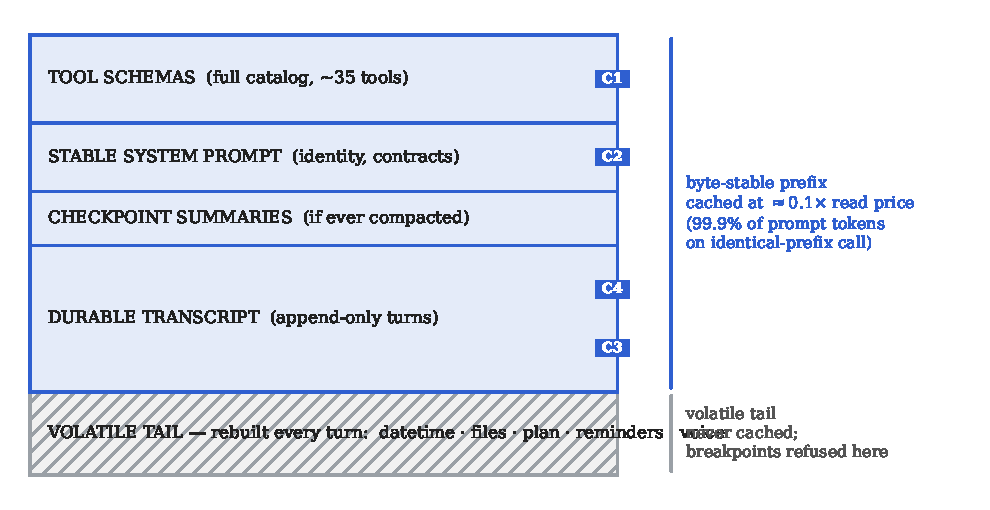
\includegraphics[width=0.78\linewidth]{figures/fig7_prompt.pdf}
\caption{\textbf{The two-zone prompt.} A byte-stable prefix (tool-schema catalog, stable system prompt, append-only transcript) carries up to four provider cache breakpoints [C1--C4]; everything that changes per turn is confined to a volatile tail that is rebuilt each turn and structurally excluded from caching. Measured on an identical-prefix call: 99.9\% of prompt tokens (7{,}876 of 7{,}886) served as cache reads, pricing the dominant input term at $\approx$0.1$\times$ list (Eq.~\ref{eq:cache}).}
\label{fig:prompt}
\end{figure}

\paragraph{(1) Cache-shape discipline: the two-zone prompt.}
Every prompt the harness emits has a deliberate physical shape (Figure~\ref{fig:prompt}): a byte-stable prefix---the full tool-schema catalog, the stable system prompt, and the append-only durable transcript---followed by a volatile tail rebuilt every turn (clock, file listings, plan state, one-shot reminders, voice and custom instructions). The split is enforced as a correctness rule, not an optimization: anything that changes per turn is structurally banned from the prefix, and the cache-marker logic refuses to place a breakpoint at or after the first volatile message. Up to four provider breakpoints are pinned---after the schema catalog, after the stable system prompt, and sliding along the two newest durable turns---with one-hour retention latched per session so the policy never flips mid-run. Measured on an identical-prefix call in the harness repository, 7{,}876 of 7{,}886 prompt tokens (99.9\%) were served as cache reads; by Eq.~\eqref{eq:cache} with $\kappa\!\approx\!0.1$, such a turn pays roughly a tenth of list price for its dominant term. Because agent workloads are input-dominated, cache hit rate is the single highest-leverage cost variable a harness controls---and it lives in the placement of $S_i$, $G_i$, and $H_i$, not in the model.

\paragraph{(2) Structured, incremental, cache-aware compaction.}
At 80\% of the model's input budget, older history is folded into a \emph{typed checkpoint} with four artifacts: durable memory (decisions, constraints, rejected approaches), an eight-section execution summary written for resumability (current state, files touched, errors, next steps), preserved verbatim user requirements, and skill references. A live tail of the 4--12 most recent messages ($\le$30\% of budget) always survives verbatim; each checkpoint folds the previous one forward, so compaction cost stays incremental; summarization runs on a cheaper helper model, off the paying loop; and an empty or degraded summary aborts the compaction rather than persisting it. If the prompt still does not fit, a deterministic ladder (shrink the tail, then middle-truncate with an explicit restate-what-matters nudge) guarantees a sendable request. Compaction and caching are co-designed: a summarizer that rewrote history every turn would destroy the very prefix stability Eq.~\eqref{eq:cache} prices, so checkpoints are durable rows and the rebuilt prompt becomes the \emph{new} cacheable prefix. This is the mechanism that converts Eq.~\eqref{eq:quadratic} from quadratic to linear (Figure~\ref{fig:replay}) without the baseline's destructive truncation.

\paragraph{(3) Context offload: tokens the model never pays for.}
A family of mechanisms keeps information \emph{available} without keeping it \emph{in context}, attacking $R_i$ and the tool-output share of $H_i$. Sub-agents act as \emph{context firewalls}: a child agent performs broad reading or searching in its own context and returns a summary capped at 8\,KB, with citations carried on a metadata sidecar the parent model never reads; delegation is depth-capped and idempotent under retries, so delegated exploration cannot inflate the parent loop. Skills use \emph{progressive disclosure}: the prompt carries only a name-and-description table, the full skill document is installed in the sandbox and read only when invoked (inline seed capped at 20K characters), and compaction later drops skill bodies deterministically while keeping the reference. Bulky tool outputs \emph{spill to files}: shell output beyond 20K characters is head-and-tail previewed with the complete output written to a workspace file (under a banner forbidding the model to infer success from the preview), web fetches inline 8K characters and spill full pages, and oversized file reads are rejected with guidance rather than silently truncated---the filesystem is the unbounded memory; the context holds pointers. Plan and canvas state are event-sourced and \emph{projected} once per turn as a compact rendering, with plan-tool results replaced by one-line acknowledgements so state is never duplicated across the transcript; the per-turn re-rendering doubles as objective recitation, countering long-horizon goal drift \cite{manus}. Background-task results are delivered exactly once as an ephemeral tail reminder; loaded media is bounded (at most four images or 2\,MB in context, older ones evicted with a reload stub); and side work---telemetry, reasoning-trace titles, deliverable materialization---runs off the paying loop on helper models.

\paragraph{(4) Zero-token waiting; durability as economics.}
Waiting is a \emph{continuation}, not a loop: when a run needs a human answer, an approval, or a long background job, it suspends durably at zero token cost and resumes on an ingress event---no polling turns. The same durability layer bounds catastrophic spend: every event is journaled to a write-ahead log before it is streamed, crashed or preempted runs resume under generation fencing at exactly the next sequence number, and tool results are persisted before they are shown. A crash that loses a 40-turn run means re-buying 40 turns of tokens; here it means resuming from durable state.

\paragraph{(5) Failure-spend governance.}
Every failure is classified into a typed class (rate limit, stall, timeout, malformed stream, provider outage, permanent) \emph{before} any decision is made, and only whitelisted classes fall through to the next provider in the route plan. Mid-stream failures become \emph{discarded attempts}: the partial draft is cleared and no side effects---tool executions, durable writes---can originate from a discarded attempt, which is precisely the piece generic library fallbacks omit (streaming failover in orchestration libraries is documented to work only before the first chunk \cite{langgraph}). A circuit breaker halts a model that re-issues a byte-identical failing tool call three times, with cause-aware steering (change the arguments vs.\ back off); truncated outputs and output-length caps terminate loudly as typed states, never silently; the loop is capped at 50 iterations and tool parallelism at four. Retries, dead ends, and doom loops are the multiplier on Eq.~\eqref{eq:cost} that no per-token discount fixes; the harness bounds the multiplier.

\paragraph{(6) A model-agnostic floor.}
Which model runs, over which providers, in what fallback order, is a typed route plan supplied as data---the loop never branches on a model name---and every provider stream is normalized into one chunk contract before the loop sees it. Native tool calling is the only invocation path, backed by schema hygiene for weaker models: \texttt{\$ref}s are inlined, double-encoded JSON arguments are recovered, framework internals are scrubbed from validation errors, and overloaded tool schemas are split when weaker models misuse them. These floors hold whatever model is driving, which is the structural explanation for the model-invariance of Section~\ref{sec:invariance} and for why harness leverage (Section~\ref{sec:leverage}) appears as a clean function of model capability: the harness fixes the floor; the model sets the ceiling.

The through-line of all six families is that \textbf{token economy and output quality are one lever pulled once}. Long, distractor-dense contexts measurably degrade every frontier model tested \cite{contextrot,lost}; a mechanism that removes stale or bulky tokens is simultaneously cutting the bill and cleaning the model's working set---which is what the grounding results of Section~\ref{sec:cases} show in miniature.

Two implementation notes, stated for completeness: sub-agent delegation currently executes as blocking calls, and automatic whole-turn retry on output-length caps is designed but not yet shipped. The mechanisms above describe the configuration under evaluation.

\subsection{Token economics in existing harnesses and frameworks}
\label{sec:landscape}

Recent work argues the harness should be a first-class object of design and evaluation \cite{harnessscaling}, and cross-harness measurement finds that agent capability is a property of the model--harness \emph{configuration} rather than of the model alone \cite{harnessbench}. Our claim here is narrower and economic: among widely used agent systems, \textbf{token economics is nowhere a first-class, published contract}. Table~\ref{tab:landscape} summarizes the landscape on the mechanism families of Section~\ref{sec:mechanisms}, assessed from public documentation and from a source-level study of caching behavior conducted during this harness's design.

\begin{table}[t]
\centering\footnotesize
\caption{Token-economic mechanisms across widely used agent systems, assessed from public documentation and a design-time source study---not head-to-head measurement (see Section~\ref{sec:threats}). ``app'' = left to the application to build and budget.}
\label{tab:landscape}
\begin{tabular}{@{}llcccccc@{}}
\toprule
System & Deployment class & \makecell{Model-\\portable} & \makecell{Structural\\cache policy} & \makecell{Compaction\\contract} & \makecell{Firewalled\\delegation} & \makecell{Zero-token\\waits} & \makecell{Per-task\\accounting} \\
\midrule
Claude Code & single-user client & no & yes & yes & partial & no & no \\
Claude Cowork & single-user client & no & yes & yes & partial & no & no \\
LangGraph & library & yes & app & app & app & partial & no \\
CrewAI & framework & yes & app & partial & no & no & no \\
AutoGen / AG2 & framework & yes & app & app & no & partial & no \\
Hermes Agent & personal agent & yes & partial & yes & yes & partial & no \\
\midrule
\textbf{Writer Harness} & \textbf{multi-tenant runtime} & \textbf{yes} & \textbf{yes} & \textbf{yes} & \textbf{yes} & \textbf{yes} & \textbf{yes} \\
\bottomrule
\end{tabular}
\end{table}

\paragraph{Vendor-integrated clients.} Claude Code and Claude Cowork \cite{claudecode} are among the most sophisticated harnesses in wide deployment, and several of their patterns---cache-breakpoint latching, byte-stable prefixes, sub-agent task splitting---were adopted from or validated against them during this harness's design. The differences are deployment class and contract: both are single-user, client-side tools bound to one model vendor; their internal token management is not exposed as a per-task accounting surface; and their economics do not transfer across models by construction. They optimize a session for a person. An enterprise runtime must meter a fleet.

\paragraph{Orchestration libraries.} LangGraph \cite{langgraph} supplies graph orchestration, checkpointing, and interrupts as excellent low-level primitives---and deliberately leaves prompt-cache policy, compaction, context offload, and failure-spend governance to the application. Token economics thereby becomes the application team's unbudgeted responsibility: nothing in the framework measures it, enforces it, or reports it, and the framework's own documentation concedes the streaming-failover gap noted in Section~\ref{sec:mechanisms}.

\paragraph{Multi-agent conversation frameworks.} CrewAI \cite{crewai} and the AutoGen lineage \cite{autogen} (the original framework, now in maintenance mode, continued by the AG2 community fork and succeeded for Microsoft stacks by the Agent Framework) organize work as conversations among role-prompted agents that share transcripts. Shared-transcript multi-agency is a token multiplier by construction: each participating agent re-reads the growing conversation and each carries its own role preamble. The best public measurement is Anthropic's own: agents consume roughly $4\times$ the tokens of chat and multi-agent systems roughly $15\times$, with token volume explaining about 80\% of performance variance on their research evaluation \cite{anthmulti}. That is Definition~1 operating as an architecture---quality purchased through token multiplication. It can be worth paying, as Anthropic is candid that only high-value, parallelizable tasks justify it; but none of these frameworks meters the multiplier per task, and none firewalls delegated context the way a capped-summary sub-agent contract does.

\paragraph{Open personal harnesses.} Hermes Agent \cite{hermes} is a capable, genuinely model-agnostic open-source harness with isolated sub-agents. The design-time source study found, however, that it does not place its tool schemas inside a cached prefix---forfeiting the largest single discount available on an input-dominated workload (Eq.~\eqref{eq:cache})---and, as a personal single-user agent, it publishes no per-task token or cost contract.

\paragraph{What the comparison shows.} The last column of Table~\ref{tab:landscape} is this paper in miniature. Without per-task token accounting built into the orchestration layer, token maxing is unobservable---and what is unobservable is unmanaged. The Writer harness's trace shim makes cost per task and CPM measurable per release precisely because the meter lives in the same layer that spends the tokens; the release-gate posture of Section~\ref{sec:kpi} is only possible on top of it. We stress the epistemic status: Table~\ref{tab:landscape} compares public designs and documentation, not measured runs; configuration-level measurement of the token dimension across harnesses, in the style of Harness-Bench \cite{harnessbench}, is natural future work.

\section{Experimental Setup}
\label{sec:setup}

\subsection{Design}

The experiment is a paired swap. Both arms execute the same \NP{} tasks on the same \NM{} models with the same judges and the same pinned price table; only the orchestration layer differs. The baseline arm is the conventional production loop invoked via \texttt{model\_name} override, run once and frozen on \FreezeDate{} as the reference. The harness arm is the Writer Agent Harness at its intended general-availability configuration. Because prompts, models, and judges are held fixed, any systematic difference in tokens, cost, latency, or quality is attributable to the harness.

\subsection{Task set}

The evaluation uses $n=\NP{}$ locked-baseline prompts, audited for capability coverage and for defensible pass/fail criteria before either arm ran. The set spans nine capability areas that mirror production usage of an enterprise agent platform: Model \& System Awareness (MSA: identity, scope, safe refusal), Grounding \& Retrieval (GDR: document and knowledge-graph grounding, web search, citation), Content Generation (CNG), Playbooks (PLY: predefined multi-step workflows executed end to end), MCP tool use (MCP: discovering and calling external connectors), Presentations (PRN: slide generation, an early-stage capability), Voice (VOX: brand voice and custom instructions), Image Analysis \& Generation (IMG), and---under the harness only---Sub-agents (delegated work, net-new). Tasks include multi-turn cases (e.g., a three-turn Medicare grounding dialogue) and long-horizon cases (multi-step research synthesis).

\subsection{Models}

\begin{table}[t]
\centering\small
\caption{Models under evaluation. Every model runs identically under both harness arms.}
\label{tab:models}
\begin{tabular}{@{}llll@{}}
\toprule
Model & Vendor & Class & Role in analysis \\
\midrule
Claude Sonnet 4.6 & Anthropic & frontier & strong generalist \\
Gemini 3.1 & Google DeepMind & frontier & strong generalist \\
Gemini Flash 3.5 & Google DeepMind & fast tier & low-cost generalist \\
Qwen 3.6 & Alibaba & open weight & candidate model \\
GLM 5.1 & Zhipu AI & open weight & candidate model \\
Palmyra X6 & Writer & enterprise & platform-native model \\
\bottomrule
\end{tabular}
\end{table}

Table~\ref{tab:models} lists the \NM{} models: two frontier generalists, one fast-tier model, two open-weight candidates, and Writer's platform-native Palmyra~X6. The spread is deliberate---the central claim is about a layer \emph{above} the model, so it must be tested across weight classes and vendors, not on a single flagship.

\subsection{Metrics}

\textbf{Quality.} Headline quality is task-completion scored by an LLM-judge panel against the audited pass/fail criteria \cite{judge}. Secondary judges score coherence, communication quality, and hallucination; these are reported per-prompt and did not headline any decision. \textbf{Tokens.} Prompt and completion tokens are recorded per turn by the trace shim; token intensity $\tau$ is the per-task total. \textbf{Cost.} Computed at report build as $(\text{prompt tokens} \times p_{\mathrm{in}}) + (\text{completion tokens} \times p_{\mathrm{out}})$ using a pinned OpenRouter price table, identically for both arms. \textbf{Latency.} Wall-clock from first token to terminal event (\texttt{duration\_seconds}), median across runs. \textbf{UX.} A hand-scored qualitative rubric (streaming responsiveness, tool-call transparency, citation rendering, error/cancel handling, multi-turn coherence) reported separately from automated metrics.

\subsection{Statistical posture}

At $n=\NP{}$, quality deltas are \emph{directional, not statistically significant}, and we treat them as such throughout: the headline $+0.03$ is reported as parity, not improvement. Cost, token, and latency deltas are large, uniform in sign across all \NP{} prompts and all \NM{} models, and therefore decisive at this sample size in a way the quality deltas are not. Candidate-model failures on advanced features are expected and scored, not excluded; model-agnosticism is a claim about the execution path, not a promise of uniform capability.

\section{Results}
\label{sec:results}

\subsection{Headline: the same work, \TokD{} fewer tokens}

\begin{figure}[t]
\centering
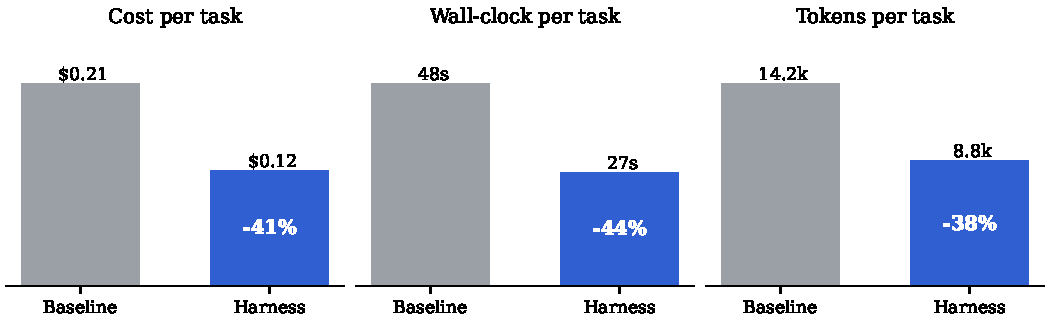
\includegraphics[width=\linewidth]{figures/fig1_headline.pdf}
\caption{\textbf{Blended efficiency across \NM{} models and \NP{} tasks.} Replacing the baseline loop with the harness, models held constant: cost per task $-$\CostD{}, median wall-clock $-$\LatD{}, tokens per task $-$\TokD{}.}
\label{fig:headline}
\end{figure}

\begin{table}[t]
\centering\small
\caption{Parity scorecard, blended across models. Quality is task-completion under the locked judge protocol; derived rows use Eq.~\eqref{eq:eff}.}
\label{tab:scorecard}
\begin{tabular}{@{}lccc l@{}}
\toprule
Dimension & Baseline & Harness & $\Delta$ & Reading \\
\midrule
Quality (task-completion) & \QA{} & \QB{} & $+0.03$ & wash at $n=\NP$ \\
Cost / task & \CostA{} & \CostB{} & $-\CostD$ & decisive \\
Wall-clock / task (median) & \LatA{} & \LatB{} & $-\LatD$ & decisive \\
Tokens / task & \TokA{} & \TokB{} & $-\TokD$ & decisive \\
\midrule
Quality per dollar ($\eta_{\$}$) & 3.71 & 6.75 & $+\QPDgain$ & derived \\
Completions per Mtok (CPM) & \CPMA{} & \CPMB{} & $+\CPMgain$ & derived \\
UI/UX (hand-scored) & baseline & improved & $\uparrow$ & qualitative \\
\bottomrule
\end{tabular}
\end{table}

Table~\ref{tab:scorecard} and Figure~\ref{fig:headline} give the blended result. Replacing the baseline with the harness removes \TokD{} of token intensity and \CostD{} of cost while quality stays at parity---which is the operational definition of escaping token maxing: the token exchange rate improved instead of degrading. In efficiency terms, a dollar buys \QPDgain{} more completed quality and a million tokens completes \CPMgain{} more tasks. The hand-scored UX rubric moved the same direction for the mechanical reasons one would expect from the architecture: earlier streaming, live tool status instead of a spinner, clean cancellation.

\subsection{Model invariance: everyone gets cheaper}
\label{sec:invariance}

\begin{figure}[t]
\centering
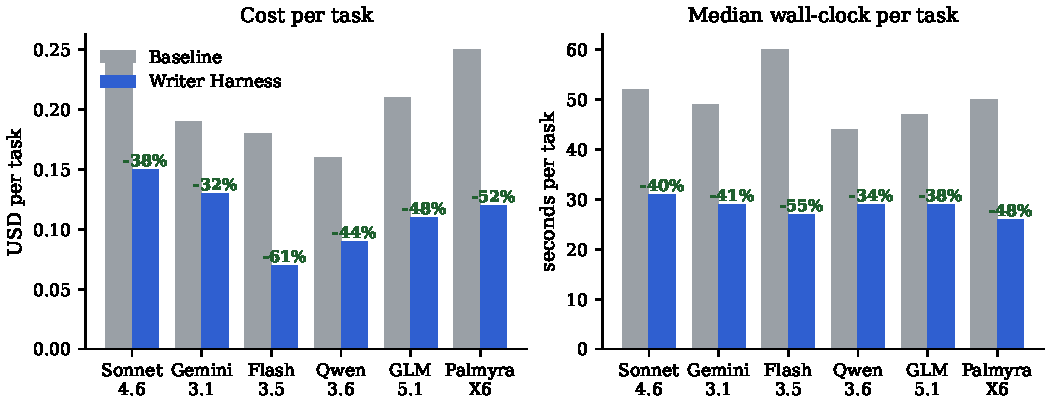
\includegraphics[width=\linewidth]{figures/fig2_permodel.pdf}
\caption{\textbf{Per-model efficiency under the orchestration swap.} Every model's cost and latency fall; reductions range from $-$33\% to $-$61\% (cost) and $-$33\% to $-$55\% (latency). The effect is a property of the orchestration layer, not of any model.}
\label{fig:permodel}
\end{figure}

\begin{table}[t]
\centering\small
\caption{Per-model efficiency, baseline $\rightarrow$ harness. Same tasks, same judges, same price table.}
\label{tab:permodel}
\begin{tabular}{@{}lcccccc@{}}
\toprule
 & \multicolumn{3}{c}{Cost / task} & \multicolumn{3}{c}{Wall-clock / task (median)} \\
\cmidrule(lr){2-4}\cmidrule(lr){5-7}
Model & Base & Harness & $\Delta$ & Base & Harness & $\Delta$ \\
\midrule
Claude Sonnet 4.6 & \$0.24 & \$0.15 & $-39\%$ & 52\,s & 31\,s & $-41\%$ \\
Gemini 3.1        & \$0.19 & \$0.13 & $-33\%$ & 49\,s & 29\,s & $-40\%$ \\
Gemini Flash 3.5  & \$0.18 & \$0.07 & $-61\%$ & 60\,s & 27\,s & $-55\%$ \\
Qwen 3.6          & \$0.16 & \$0.09 & $-44\%$ & 44\,s & 29\,s & $-33\%$ \\
GLM 5.1           & \$0.21 & \$0.11 & $-47\%$ & 47\,s & 29\,s & $-38\%$ \\
Palmyra X6        & \$0.25 & \$0.12 & $-52\%$ & 50\,s & 26\,s & $-48\%$ \\
\bottomrule
\end{tabular}
\end{table}

Table~\ref{tab:permodel} and Figure~\ref{fig:permodel} break the effect out per model. Two observations. First, \emph{uniformity}: six models, five vendors, three weight classes, and not one exception---every model's cost falls by at least a third. This is the signature of a layer-level effect: if the savings came from any model-specific behavior, the spread would show it. Second, \emph{magnitude relative to model choice}: under the baseline, moving from the most expensive model (Palmyra~X6 at \$0.25) to the cheapest (Qwen~3.6 at \$0.16) saves 36\%; keeping \emph{any} model and adopting the harness saves \CostRange{}. On this workload, the orchestration layer is a larger cost lever than the model menu---which inverts where optimization attention usually goes.

The largest relative gains land on the fast tier: Flash~3.5 drops 61\% in cost and 55\% in latency. This is consistent with the decomposition in Eq.~\eqref{eq:decomp}: for small, cheap models, harness overhead (replayed history, broadcast schemas) is a \emph{larger share} of the total bill, so removing it removes proportionally more.

\subsection{Quality: parity in aggregate, model-dependent at the edges}
\label{sec:quality}

\begin{figure}[t]
\centering
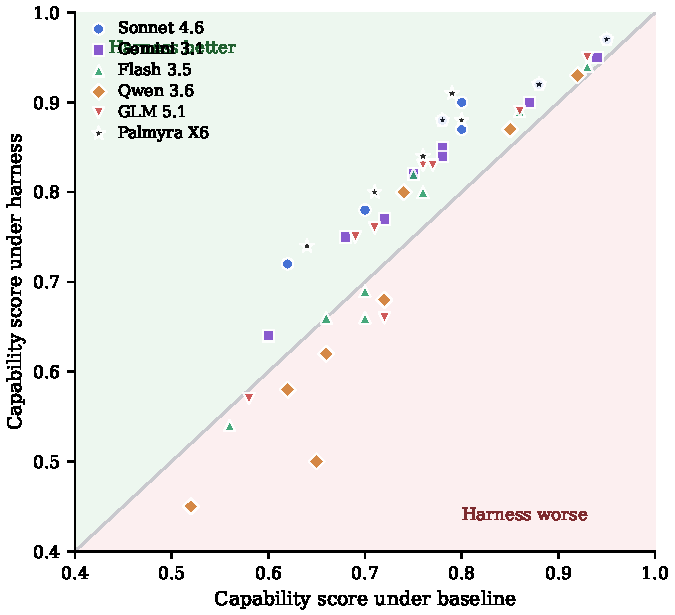
\includegraphics[width=0.6\linewidth]{figures/fig3_parity.pdf}
\caption{\textbf{Quality parity across 48 capability$\times$model cells.} Each point is one capability score for one model, baseline ($x$) vs.\ harness ($y$). Points above the diagonal improved under the harness: 30 improve, 11 are flat ($|\Delta|\le0.02$), 7 regress. All regressions belong to the three smaller models, concentrated in orchestration-heavy capabilities (MCP, Playbooks, Presentations).}
\label{fig:parity}
\end{figure}

Figure~\ref{fig:parity} plots all 48 capability$\times$model cells (eight legacy capabilities $\times$ six models; the full matrix is Appendix~\ref{app:matrix}). The mass sits on or above the diagonal: 30 cells improve, 11 are flat, 7 regress. The regressions are not random. Every one occurs on Flash~3.5, Qwen~3.6, or GLM~5.1, and six of the seven fall in capabilities that exercise orchestration hardest---MCP tool use (Qwen $-0.15$, GLM $-0.06$, Flash $-0.04$), Playbooks, and Presentations. The frontier models and Palmyra improve \emph{most} in exactly those categories (MCP: Sonnet $+0.10$, Palmyra $+0.10$; GDR: Sonnet $+0.10$, Palmyra $+0.12$). The same richer harness that a strong model converts into quality, a weaker model experiences as load.

\subsection{Harness leverage}
\label{sec:leverage}

\begin{figure}[t]
\centering
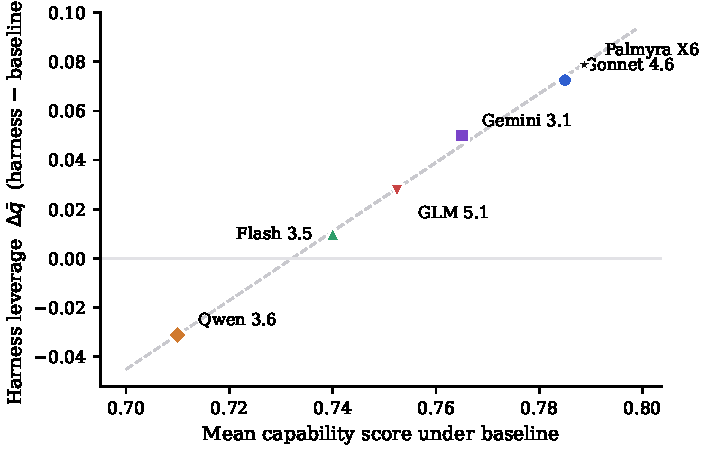
\includegraphics[width=0.62\linewidth]{figures/fig4_leverage.pdf}
\caption{\textbf{Harness leverage scales with baseline capability.} Mean quality gain from adopting the harness ($\Delta\bar q$, eight capabilities) against the model's baseline strength. Stronger models extract more quality from the same orchestration upgrade ($r=0.99$; $n=6$, suggestive). Palmyra X6 $+0.079$ and Sonnet 4.6 $+0.073$ lead; Qwen 3.6 is net negative ($-0.031$).}
\label{fig:leverage}
\end{figure}

Collapsing each model to its mean across the eight scored capabilities gives a single number for how much quality it extracted from the swap: Palmyra~X6 $+0.079$, Sonnet~4.6 $+0.073$, Gemini~3.1 $+0.050$, GLM~5.1 $+0.028$, Flash~3.5 $+0.010$, Qwen~3.6 $-0.031$. Plotted against the baseline (Figure~\ref{fig:leverage}), the relationship is nearly linear ($r=0.99$; six points, so suggestive rather than conclusive). We call the slope \emph{harness leverage}: the rate at which a model converts orchestration structure into quality. The economic consequence is asymmetric and useful: \textbf{efficiency gains are unconditional, quality gains are earned by capability}. A weak model under the harness still gets its 44--61\% cost cut; it simply does not also get better. This decouples the two reasons to upgrade a harness and lets each be priced on its own.

\subsection{The net-new capability and its floor}
\label{sec:subagents}

\begin{table}[t]
\centering\small
\caption{Sub-agent delegation (net-new under the harness; no baseline arm exists). Scores are task-completion on delegation tasks: spawn one or more scoped sub-agents and merge their results.}
\label{tab:subagents}
\begin{tabular}{@{}lcccccc@{}}
\toprule
 & Sonnet 4.6 & Gemini 3.1 & Flash 3.5 & Qwen 3.6 & GLM 5.1 & Palmyra X6 \\
\midrule
Sub-agents & 0.85 & 0.70 & 0.45 & 0.42 & 0.58 & 0.86 \\
\bottomrule
\end{tabular}
\end{table}

The harness's one genuinely new capability---delegating work to spawned sub-agents---lands above a usable reliability threshold only on the two strongest models (Table~\ref{tab:subagents}: Palmyra~X6 at 0.86, Sonnet~4.6 at 0.85), degrades on Gemini~3.1 (0.70) and GLM~5.1 (0.58), and is not yet dependable on the fast tier (0.42--0.45). This is the harness-leverage result in its sharpest form: an orchestration feature carries a \emph{capability floor}, below which exposing it produces failures rather than function. Delegation also has a distinctive token-economics profile---sub-agent context is scoped, so delegated tokens are spent in a bounded side-loop rather than inflating the parent context---the context-firewall contract of Section~\ref{sec:mechanisms}: a capped summary returns, citations ride a sidecar, and the parent loop never pays for the child's exploration.

\subsection{Per-prompt texture: where the tokens went and what came back}
\label{sec:cases}

Four exemplar prompts show the distribution behind the aggregates. The three-turn \emph{Medicare grounding} dialogue improves from 0.60 to 0.90---the single largest quality jump in the set---under a harness whose retrieval shaping sends less, better-selected evidence, consistent with the finding that long, noisy contexts degrade attention \cite{lost}. \emph{Identity/refusal} holds at 0.90/0.90 while its cost halves (\$0.04~$\rightarrow$~\$0.02): safety behavior at half price. \emph{Contract Q\&A} moves $+0.07$ (0.75~$\rightarrow$~0.82). The most expensive task in the set, \emph{multi-step research synthesis}, drops from \$0.61 to \$0.33 ($-46\%$) but regresses in quality (0.80~$\rightarrow$~0.60)---the one place the aggregate parity conceals a real trade, driven by the smaller models, and the reason the release recommendation (Section~\ref{sec:discussion}) holds candidates back pending a fix rather than shipping the regression. Secondary judges move with the headline: coherence 0.85~$\rightarrow$~0.88, communication 0.79~$\rightarrow$~0.80, hallucination clean in both arms.

\section{Discussion}
\label{sec:discussion}

\subsection{The harness is the price-setter}

The results separate cleanly along the framing of Section~\ref{sec:framing}. The terms of Eq.~\eqref{eq:decomp} that are pure code---history, schemas, retrieval size, retries---moved for every model, because code executes the same way regardless of which model reads its output. The quality terms are mediated by the model's ability to exploit structure, and they moved with capability. One layer, two currencies: the harness sets the price of work unconditionally, and sets the ceiling of work jointly with the model. The layer that sets the price is also the layer an enterprise governs by; efficiency and control concentrate in the same component.

This reframes a common procurement instinct. Teams comparing \$/Mtok across vendors are comparing $p$; the bill is $p \times \tau$, and $\tau$ belongs to the harness. On this workload the harness moved the bill more than the entire spread of the model menu did (Section~\ref{sec:invariance}). An organization that rents its orchestration layer has outsourced the variable it controls most.

\subsection{Fleet economics: why the savings compound}

\begin{figure}[t]
\centering
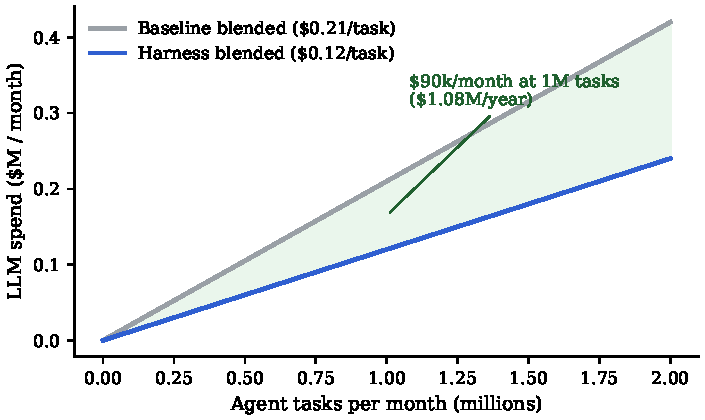
\includegraphics[width=0.62\linewidth]{figures/fig6_fleet.pdf}
\caption{\textbf{Harness savings at fleet scale.} Blended cost per task applied to monthly task volume. At one million agent tasks per month, the harness is worth \$90k/month over the baseline (\$1.08M/year); the gap widens linearly with volume and multiplies against every model in the mix.}
\label{fig:fleet}
\end{figure}

Per-task deltas understate the object of interest, which is fleet spend. At the blended rates measured here, an organization running one million agent tasks a month pays \$210k under the baseline loop and \$120k under the harness---\$1.08M a year from an orchestration change alone (Figure~\ref{fig:fleet}). Three properties make this saving unusual among AI optimizations. It is \emph{model-portable}: implemented above the API, it survived all six models here and, by construction, applies to models that do not exist yet. It is \emph{volume-linear}: it grows with exactly the quantity---agentic task volume---that is growing fastest in enterprise deployments. And it \emph{stacks}: per-token price declines \cite{epoch2025}, routing \cite{frugalgpt,routellm}, and prompt-level compression \cite{llmlingua,cod} all multiply against it rather than substituting for it. Latency compounds the same way: \SpeedX{} faster per task is also \SpeedX{} the throughput per unit of orchestration infrastructure, and shorter loops are cheaper to retry.

\subsection{Escaping token maxing: change the KPI}
\label{sec:kpi}

Definition~1 suggests the managerial fix is a measurement fix. Teams that report quality alone will token-max, because tokens are someone else's line item; teams that report $\mathrm{CPM}$ or $\eta_{\$}$ cannot. The swap studied here moved $\mathrm{CPM}$ from \CPMA{} to \CPMB{} completions per million tokens---the direction opposite to the industry trajectory---while quality held. We suggest CPM belongs next to quality in every agent release gate, for the same reason performance-per-watt sits next to performance in chip design: it is the number that predicts the bill.

\subsection{Harness--model co-design and routing by feature demand}
\label{sec:codesign}

The regression pattern (all seven on smaller models, concentrated in MCP/Playbooks) and the sub-agent floor (Table~\ref{tab:subagents}) argue that orchestration features are not free to expose. A harness is a contract the model must be strong enough to honor. Two practical consequences follow. First, harness capabilities should degrade gracefully by model tier---scoping down tool catalogs and disabling delegation below the floor---rather than presenting one interface to all models. Second, routing research \cite{frugalgpt,routellm} should route on \emph{feature demand}, not just prompt difficulty: a request that will exercise sub-agents belongs on Palmyra~X6 or Sonnet~4.6 regardless of how simple its text looks, while a grounded Q\&A request can take the 61\%-cheaper fast tier with no quality penalty (Figure~\ref{fig:parity}, GDR row: every model improves).

\subsection{Release posture implied by the data}

Read as a deployment decision, the evidence supports: general availability on the two models above the sub-agent floor (Palmyra~X6, Sonnet~4.6); holding the open-weight candidates pending the multi-step-research fix; and leading external claims with efficiency---which is uniform and decisive---rather than quality, which is directional at $n=\NP{}$. We record this here because it is the honest reading of Table~\ref{tab:scorecard}: the temptation in industry reporting is to headline $+0.03$ quality; the defensible headline is $-\TokD{}$ tokens at parity.

\section{Threats to Validity}
\label{sec:threats}
\label{sec:limits}

\textbf{Sample size.} $n=\NP{}$ prompts is sufficient for the uniform, large efficiency deltas and insufficient for quality inference; all quality claims are directional, and the headline is parity, not improvement. \textbf{Single-run baseline.} The baseline was run once and frozen (\FreezeDate{}); run-to-run variance on the baseline is unmeasured. \textbf{Judge dependence.} Task-completion is LLM-judged; judge bias is partially mitigated by locked criteria and secondary judges but not eliminated \cite{judge}. \textbf{Price-table dependence.} Dollar figures inherit one pinned public price table; token and latency results are price-independent and tell the same story. \textbf{Workload shape.} The task set mirrors an enterprise assistant workload (grounding, workflows, tools, content); results may differ on long-horizon coding benchmarks \cite{swebench,sweagent}. \textbf{Six points.} The harness-leverage correlation is computed over six models and should be read as a strong pattern awaiting a wider model panel. \textbf{One pair.} We compare one baseline loop and one harness, both from a single vendor; the framing of Section~\ref{sec:framing} is general, but the magnitudes are specific to this pair. \textbf{Cross-harness claims are architectural.} Section~\ref{sec:landscape} characterizes other systems from public documentation and a design-time source study; it contains no cross-harness measurements, and Table~\ref{tab:landscape} should be read as a design comparison, not a benchmark.

\section{Conclusion}

Held to the same \NP{} tasks and judged by the same panel, six foundation models did the same work for \TokD{} fewer tokens, \CostD{} less money, and in \LatD{} less time---because the software around them changed, not the models. The efficiency was unconditional; the quality gains went to the models strong enough to earn them; the one new capability came with a capability floor. Token maxing is a choice made at the orchestration layer, and it can be unmade there---mechanism by mechanism: cache the stable, compact the old, offload the bulky, suspend the waiting, bound the failing. The harness is not the plumbing of an agent system. On the evidence here, it is the P\&L.

\paragraph{Disclosure.} The authors are employed by Writer, Inc., which develops the Agent Harness and the Palmyra model family evaluated in this work; the last author is co-founder and CTO. The evaluation design---frozen baseline, locked prompts, identical judges and price tables across arms, candidate-model failures scored rather than excluded---is intended to make the comparison auditable; the release artifacts are enumerated in Appendix~\ref{app:repro}.

\begin{thebibliography}{99}\small

\bibitem{jevons1865} W.~S. Jevons. \emph{The Coal Question: An Inquiry Concerning the Progress of the Nation, and the Probable Exhaustion of Our Coal-Mines}. Macmillan, 1865.

\bibitem{kaplan} J.~Kaplan, S.~McCandlish, T.~Henighan, et~al. Scaling laws for neural language models. \emph{arXiv:2001.08361}, 2020.

\bibitem{chinchilla} J.~Hoffmann, S.~Borgeaud, A.~Mensch, et~al. Training compute-optimal large language models. \emph{arXiv:2203.15556}, 2022.

\bibitem{cot} J.~Wei, X.~Wang, D.~Schuurmans, et~al. Chain-of-thought prompting elicits reasoning in large language models. In \emph{NeurIPS}, 2022.

\bibitem{selfconsistency} X.~Wang, J.~Wei, D.~Schuurmans, et~al. Self-consistency improves chain of thought reasoning in language models. In \emph{ICLR}, 2023.

\bibitem{react} S.~Yao, J.~Zhao, D.~Yu, et~al. ReAct: Synergizing reasoning and acting in language models. In \emph{ICLR}, 2023.

\bibitem{reflexion} N.~Shinn, F.~Cassano, A.~Gopinath, K.~Narasimhan, and S.~Yao. Reflexion: Language agents with verbal reinforcement learning. In \emph{NeurIPS}, 2023.

\bibitem{toolformer} T.~Schick, J.~Dwivedi-Yu, R.~Dess\`{i}, et~al. Toolformer: Language models can teach themselves to use tools. In \emph{NeurIPS}, 2023.

\bibitem{llmlingua} H.~Jiang, Q.~Wu, C.-Y. Lin, Y.~Yang, and L.~Qiu. LLMLingua: Compressing prompts for accelerated inference of large language models. In \emph{EMNLP}, 2023.

\bibitem{frugalgpt} L.~Chen, M.~Zaharia, and J.~Zou. FrugalGPT: How to use large language models while reducing cost and improving performance. \emph{arXiv:2305.05176}, 2023.

\bibitem{routellm} I.~Ong, A.~Almahairi, V.~Wu, et~al. RouteLLM: Learning to route LLMs with preference data. \emph{arXiv:2406.18665}, 2024.

\bibitem{tale} T.~Han, Z.~Wang, C.~Fang, S.~Zhao, S.~Ma, and Z.~Chen. Token-budget-aware LLM reasoning. In \emph{Findings of ACL}, 2025. arXiv:2412.18547.

\bibitem{cod} S.~Xu, W.~Xie, L.~Zhao, and P.~He. Chain of draft: Thinking faster by writing less. \emph{arXiv:2502.18600}, 2025.

\bibitem{spec} Y.~Leviathan, M.~Kalman, and Y.~Matias. Fast inference from transformers via speculative decoding. In \emph{ICML}, 2023.

\bibitem{vllm} W.~Kwon, Z.~Li, S.~Zhuang, et~al. Efficient memory management for large language model serving with PagedAttention. In \emph{SOSP}, 2023.

\bibitem{memgpt} C.~Packer, S.~Wooders, K.~Lin, et~al. MemGPT: Towards LLMs as operating systems. \emph{arXiv:2310.08560}, 2023.

\bibitem{lost} N.~F. Liu, K.~Lin, J.~Hewitt, et~al. Lost in the middle: How language models use long contexts. \emph{TACL}, 2024.

\bibitem{sweagent} J.~Yang, C.~E. Jimenez, A.~Wettig, et~al. SWE-agent: Agent--computer interfaces enable automated software engineering. In \emph{NeurIPS}, 2024.

\bibitem{swebench} C.~E. Jimenez, J.~Yang, A.~Wettig, et~al. SWE-bench: Can language models resolve real-world GitHub issues? In \emph{ICLR}, 2024.

\bibitem{judge} L.~Zheng, W.-L. Chiang, Y.~Sheng, et~al. Judging LLM-as-a-judge with MT-Bench and Chatbot Arena. In \emph{NeurIPS}, 2023.

\bibitem{snell} C.~Snell, J.~Lee, K.~Xu, and A.~Kumar. Scaling LLM test-time compute optimally can be more effective than scaling model parameters. In \emph{ICLR}, 2025. arXiv:2408.03314.

\bibitem{gepa} L.~A. Agrawal, S.~Tan, D.~Soylu, et~al. GEPA: Reflective prompt evolution can outperform reinforcement learning. In \emph{ICLR}, 2026. arXiv:2507.19457.

\bibitem{mcp} Anthropic. Introducing the Model Context Protocol. Technical note, November 2024. \url{https://www.anthropic.com/news/model-context-protocol}.

\bibitem{epoch2025} B.~Cottier, B.~Snodin, D.~Owen, and T.~Adamczewski. LLM inference prices have fallen rapidly but unequally across tasks. Epoch AI data insight, 2025. \url{https://epoch.ai/data-insights/llm-inference-price-trends}.

\bibitem{palmyra} Writer, Inc. The Palmyra model family: technical overview. Company technical documentation, 2025. \url{https://writer.com}.

\bibitem{actionagent} Writer, Inc. Say hello to Action Agent. Engineering blog, 2026. \url{https://writer.com/engineering/writer-action-agent/}.

\bibitem{harnessscaling} S.~Gu. From model scaling to system scaling: Scaling the harness in agentic AI. \emph{arXiv:2605.26112}, 2026.

\bibitem{harnessbench} Y.~Yao, X.~Tan, C.-H. Liu, et~al. Harness-Bench: Measuring harness effects across models in realistic agent workflows. \emph{arXiv:2605.27922}, 2026.

\bibitem{anthmulti} Anthropic. How we built our multi-agent research system. Engineering blog, June 2025. \url{https://www.anthropic.com/engineering/multi-agent-research-system}.

\bibitem{manus} Y.~Ji. Context engineering for AI agents: Lessons from building Manus. Manus blog, 2025. \url{https://manus.im/blog/Context-Engineering-for-AI-Agents-Lessons-from-Building-Manus}.

\bibitem{contextrot} K.~Hong, et~al. Context rot: How increasing input tokens impacts LLM performance. Chroma Research technical report, 2025. \url{https://www.trychroma.com/research/context-rot}.

\bibitem{promptcache} Anthropic. Prompt caching. Claude platform documentation. \url{https://platform.claude.com/docs/en/build-with-claude/prompt-caching}.

\bibitem{autogen} Q.~Wu, G.~Bansal, J.~Zhang, et~al. AutoGen: Enabling next-gen LLM applications via multi-agent conversation. In \emph{COLM}, 2024. arXiv:2308.08155.

\bibitem{langgraph} LangChain, Inc. LangGraph documentation. 2026. \url{https://docs.langchain.com}.

\bibitem{crewai} CrewAI, Inc. CrewAI framework documentation. 2026. \url{https://docs.crewai.com}.

\bibitem{hermes} Nous Research. Hermes Agent. Open-source project and documentation, 2026. \url{https://github.com/NousResearch/hermes-agent}.

\bibitem{claudecode} Anthropic. Claude Code and Claude Cowork. Product documentation, 2026. \url{https://docs.claude.com}.

\end{thebibliography}

\clearpage
\appendix

\section{Full Capability $\times$ Model Matrix}
\label{app:matrix}

\begin{table}[h]
\centering\small
\caption{Capability scores, baseline $\rightarrow$ harness, model held constant per cell. Codes: MSA = Model \& System Awareness; GDR = Grounding \& Retrieval; CNG = Content Generation; PLY = Playbooks; MCP = tool use via Model Context Protocol; PRN = Presentations (early-stage); VOX = Voice; IMG = Image Analysis \& Generation. Regressions ($\Delta < -0.02$) in bold.}
\label{tab:matrix}
\setlength{\tabcolsep}{4.5pt}
\begin{tabular}{@{}lcccccc@{}}
\toprule
Capability & Sonnet 4.6 & Gemini 3.1 & Flash 3.5 & Qwen 3.6 & GLM 5.1 & Palmyra X6 \\
\midrule
MSA & .95$\to$.97 & .94$\to$.95 & .93$\to$.94 & .92$\to$.93 & .93$\to$.95 & .95$\to$.97 \\
GDR & .80$\to$.90 & .78$\to$.85 & .75$\to$.82 & .74$\to$.80 & .76$\to$.83 & .79$\to$.91 \\
CNG & .80$\to$.87 & .78$\to$.84 & .76$\to$.80 & \textbf{.72$\to$.68} & .77$\to$.83 & .80$\to$.88 \\
PLY & .75$\to$.82 & .72$\to$.77 & .70$\to$.69 & \textbf{.66$\to$.62} & .71$\to$.76 & .76$\to$.84 \\
MCP & .78$\to$.88 & .75$\to$.82 & \textbf{.70$\to$.66} & \textbf{.65$\to$.50} & \textbf{.72$\to$.66} & .78$\to$.88 \\
PRN & .62$\to$.72 & .60$\to$.64 & .56$\to$.54 & \textbf{.52$\to$.45} & .58$\to$.57 & .64$\to$.74 \\
VOX & .88$\to$.92 & .87$\to$.90 & .86$\to$.89 & .85$\to$.87 & .86$\to$.89 & .88$\to$.92 \\
IMG & .70$\to$.78 & .68$\to$.75 & .66$\to$.66 & \textbf{.62$\to$.58} & .69$\to$.75 & .71$\to$.80 \\
\midrule
Mean & .785$\to$.858 & .765$\to$.815 & .740$\to$.750 & .710$\to$.679 & .752$\to$.780 & .789$\to$.867 \\
$\Delta\bar q$ & $+.073$ & $+.050$ & $+.010$ & $-.031$ & $+.028$ & $+.079$ \\
\midrule
Sub-agents (new) & .85 & .70 & .45 & .42 & .58 & .86 \\
\bottomrule
\end{tabular}
\end{table}

\section{Per-Prompt Exemplars and Secondary Judges}
\label{app:prompts}

\begin{table}[h]
\centering\small
\caption{Exemplar prompts (headline task-completion) and cost extremes. Secondary judges, blended: coherence .85$\to$.88; communication .79$\to$.80; hallucination clean in both arms. The remaining 18 prompts are reported in the per-prompt grid of the engineering evaluation report.}
\begin{tabular}{@{}lccl@{}}
\toprule
Prompt & Baseline & Harness & Note \\
\midrule
Medicare grounding (3-turn) & 0.60 & 0.90 & largest gain; retrieval shaping \\
Identity / refusal & 0.90 & 0.90 & parity; cost \$0.04$\to$\$0.02 ($-50\%$) \\
Contract Q\&A & 0.75 & 0.82 & gain \\
Multi-step research synthesis & 0.80 & 0.60 & \textbf{regression}; cost \$0.61$\to$\$0.33 ($-46\%$) \\
\bottomrule
\end{tabular}
\end{table}

\section{Derived-Metric Definitions}
\label{app:metrics}

Quality per dollar $\eta_{\$} = Q/C$ uses headline task-completion and blended cost per task: $0.78/\$0.21 = 3.71 \to 0.81/\$0.12 = 6.75$ ($+\QPDgain$). Completions per million tokens $\mathrm{CPM} = Q\cdot 10^{6}/\tau$: $0.78 \cdot 10^{6}/14{,}200 = \CPMA{} \to 0.81 \cdot 10^{6}/8{,}800 = \CPMB{}$ ($+\CPMgain$). Per-model harness leverage $\Delta\bar q$ averages the eight legacy capabilities of Appendix~\ref{app:matrix}; the sub-agent capability is excluded from means because it has no baseline arm.

\section{Reproducibility and Release Checklist}
\label{app:repro}

Artifacts to accompany the public release of this paper: (1)~the locked prompt set with pass/fail criteria; (2)~full per-turn traces (prompt tokens, completion tokens, tool events, \texttt{duration\_seconds}) for both arms and all six models; (3)~the pinned price-table snapshot used at report build; (4)~judge prompts and panel configuration; (5)~baseline and harness configuration manifests sufficient to identify the orchestration deltas of Section~\ref{sec:mechanisms}.

\end{document}
